
\section{Results}
% \quickwordcount{03.5_results}

\subsection*{BOLD fMRI Simulations}

Figure \ref{fig:uncertainty1} illustrates the accuracy and stability of signal changes when simulating a GRE sequence in phantoms with a FoV of 1\,mm, filled with cylinders of various radii and scaled to simulate a phantom filled with 8\,µm radius cylinders. The vertical dashed line represents the mean signal change in phantoms originally filled with cylinder of radius 8\,µm, serving as the true mean in this evaluation. Error bars denote 95\% confidence intervals; they are green if overlapping the true mean and orange if not. For cylinders with initially very large or very small radii, the confidence intervals do not overlap the true mean that was determined from a simulation with a cylinder with a radius of 8\,µm. This suggests that such a re-scaling approach may not mimic the behavior of an 8\,µm cylinder through the FoV scaling approach in the current form.

%TC:ignore 
\begin{figure*}[!htbp]
    \centering
    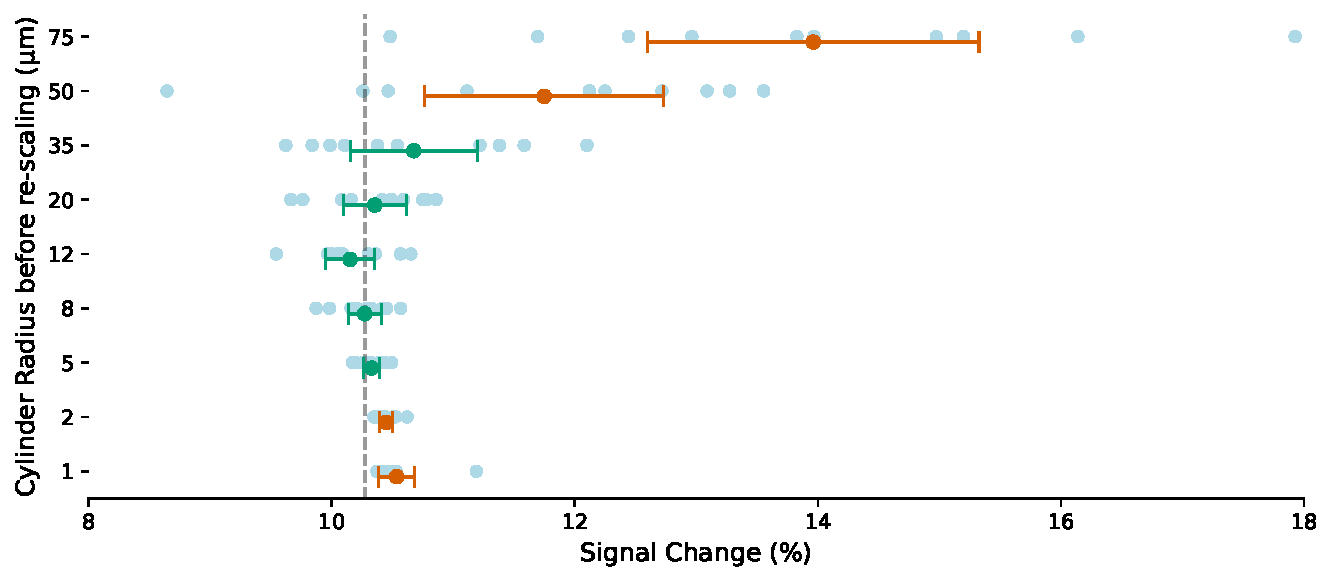
\includegraphics[width=\textwidth]{fig1_uncertainty1.pdf}
    \caption{Evaluating accuracy and stability of the FoV scaling approach. Ten phantom with a FoV of 1000\,µm and a grid size of 1000 were created, each filled with randomly positioned cylinders of specific sizes. The cylinder sizes were 1, 2, 5, 8, 12, 20, 35, 50, and 75\,µm, resulting in a total of 90 phantoms. All phantoms were set with a volume fraction of 4\%. Using FoV scaling, these phantoms were adjusted to represent a phantom filled with 8\,µm cylinders, and signal changes under GRE sequence were simulated in these environments under both active and rest conditions. The mean and 95\% confidence intervals are shown as error bars for each cylinder radius. The average result for phantoms originally containing cylinders with radii of 8\,µm was used as the reference mean, indicated by a vertical dashed line.}
    \label{fig:uncertainty1}
\end{figure*}
%TC:endignore 


In the case of a 75\,µm cylinder, FoV of the original phantom is expanded from 1000\,µm to 2000\,µm and 4000\,µm. As a result, the confidence interval narrows, and it overlaps with the true mean (Figure \ref{fig:uncertainty2}.A). When the cylinder size is not significantly smaller than the FoV (e.g., 75\,µm vs. 1\,mm) and the volume fraction is low (e.g., 4\%), only a small portion of a cylinder may fit within the phantom. Particles diffusing across the FoV might not experience the full characteristics of that cylinder. Additionally, the random placement of this partial cylinder in the phantom can introduce bias in the results. This effect can be mitigated by using a larger FoV, which may accommodate a complete cylinder rather than just a partial segment, thereby reducing the bias and providing more accurate results.

A similar result is observed when examining phantoms filled with 1\,µm cylinders, but with a different adjustment. Here, maintaining a constant FoV but increasing the grid size to achieve smaller voxels in the discrete space tightens the confidence interval and brings it closer to the true mean (Figure \ref{fig:uncertainty2}.B). A phantom with a grid size of 1\,µm or larger is not an ideal setup for accommodating cylinders of the same size or smaller, as there are not enough voxels to accurately represent the cylinders and their corresponding off-resonance maps. This issue becomes even more pronounced when the step size is comparable to the cylinder and grid size (in this study, the step size was 0.316\,µm for each dimension). Under these conditions, particles can cross vessels in just a few steps, which prevents them from adequately experiencing the dynamics of the local field inhomogeneities created by the presence of the cylinders.

%TC:ignore 
\begin{figure*}[!htbp]
    \centering
    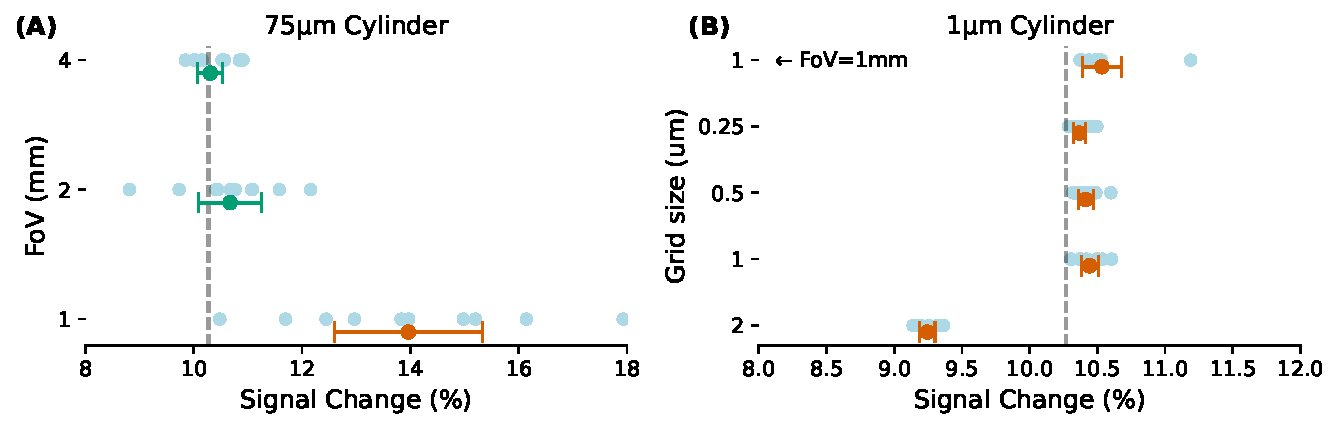
\includegraphics[width=\textwidth]{fig2_uncertainty2.pdf}
    \caption{The impact of the grid size and the original FoV on the accuracy and stability of the FoV scaling approach is evaluated. \textbf{A)} Phantoms with FoVs of 1, 2, and 4\,mm were generated, containing randomly positioned cylinders of size 75\,µm, with ten phantoms created for each FoV. \textbf{B)} Phantoms with a FoV of 500\,µm were generated with grid sizes of 0.25, 0.5, 1, and 2\,µm, each filled with randomly positioned cylinders of size 1\,µm, with ten phantoms created for each grid size. Using the FoV scaling approach, these phantoms were scaled to represent a phantom filled with 8\,µm cylinders, and the same simulations and analyses as presented in Figure \ref{fig:uncertainty1} were performed. This analysis explores how grid size and FoV affect the convergence of results for small and large cylinders, respectively. In \textbf{(A)}, increasing the FoV reduces the confidence interval, bringing it closer to the true mean for large cylinders. In \textbf{(B)}, a smaller grid size is observed to reduce the confidence interval, bringing it closer to the true mean for small cylinders. A 1\,µm grid size with a 1\,mm FoV, as presented in Figure \ref{fig:uncertainty1}, is added for comparison. True mean is taken from the analysis presented in Figure \ref{fig:uncertainty1}.}
    \label{fig:uncertainty2}
\end{figure*}
%TC:endignore 

Figure \ref{fig:BVF} illustrates the BOLD signal change in GRE, SE, and pass-band bSSFP sequences as a function of vessel radius for different BVF values ranging from 1\% to 6\%. This figure shows that SpinWalk can replicate the results shown in Figure 1 of \cite{baez2017impact}. The sensitivity of the GRE sequence remains consistent for larger vessels and is non-specific for vessels larger than approximately 6 µm. In contrast, the SE sequence shows selective sensitivity, peaking around 4 µm vessels. These findings are in line with previous results of (\cite{baez2017impact, boxerman1995mr, weisskoff1994microscopic}). While the bSSFP profile is also selective to vessel size, it is broader in comparison to the profile of the SE. The time required to generate data for a single plot (with 50 cylinder radii and two oxygenation levels) was 11.4 ± 2.8 seconds for GRE, 12.1 ± 3 seconds for SE, and 2177 ± 125 seconds for bSSFP. This duration encompasses the total run-time, including all computations, data loading, and result exporting to disk.


%TC:ignore 
\begin{figure*}[!htbp]
    \centering
    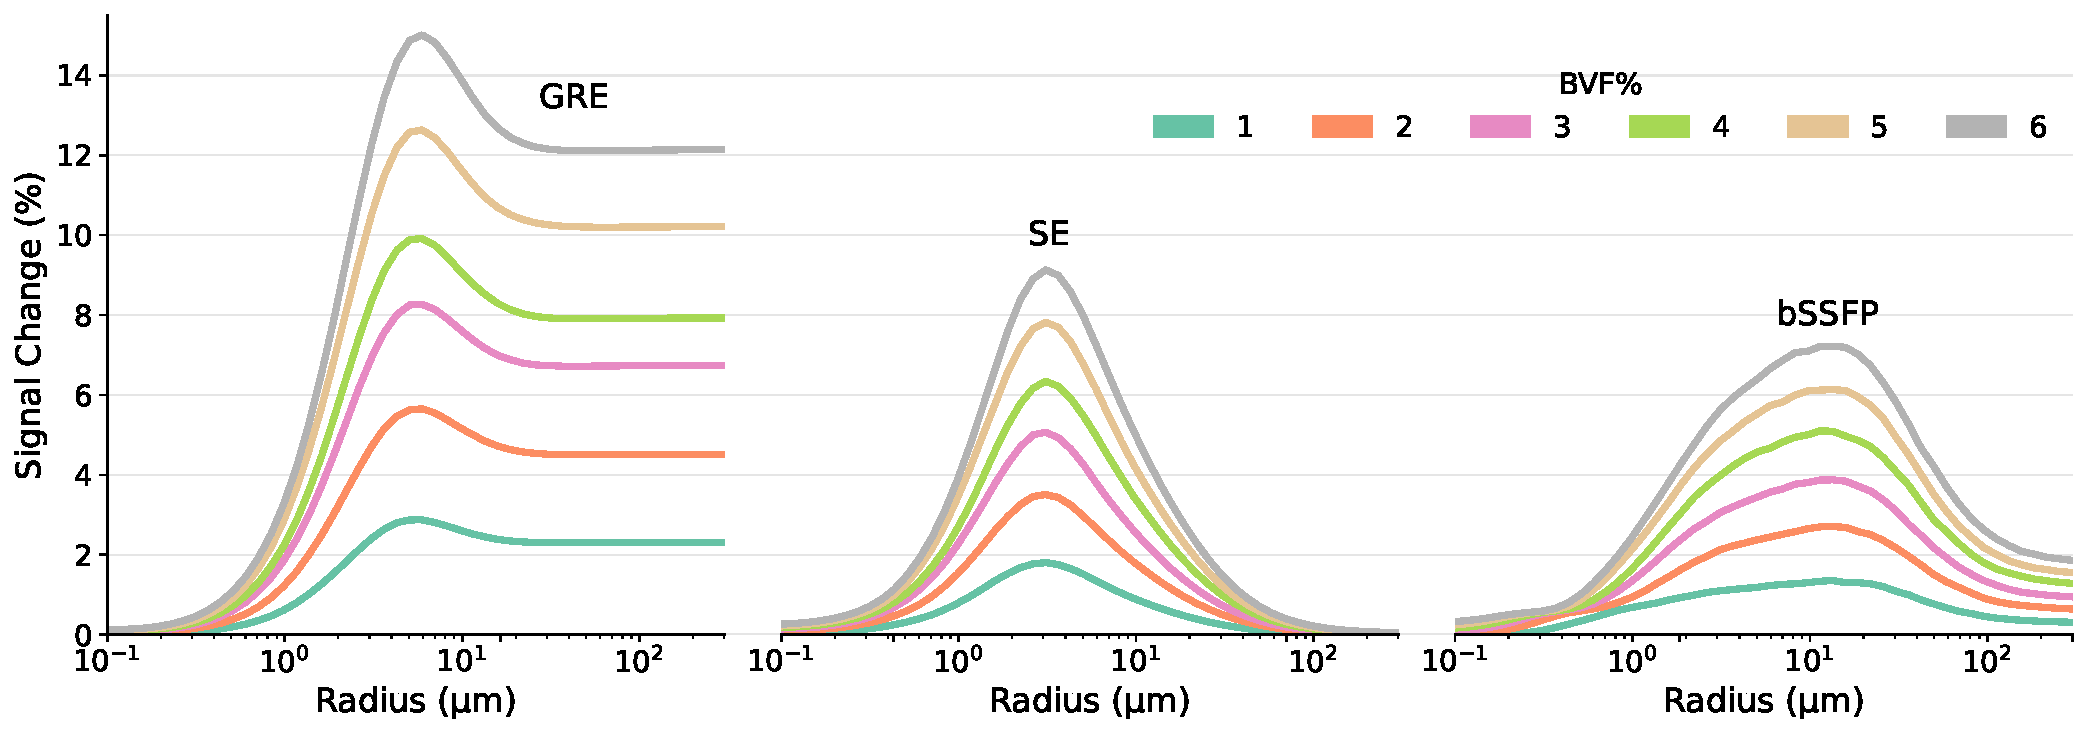
\includegraphics[width=\textwidth]{fig3_BVF.pdf}
    \caption{\protect Extravascular BOLD signal change as a function of vessel radius and blood volume fraction was examined under GRE, SE, and bSSFP sequences. Vessels were modeled as cylinders oriented perpendicular to the B\textsubscript{0} direction within a space that has a FoV of 600\,µm, a grid size of 1200, and impermeable surfaces. Blood oxygenation levels of 77\% for the resting state and 85\% for the activated state were assumed. A magnetic field strength of 9.4T is assumed for B\textsubscript{0}. }
    \label{fig:BVF}
\end{figure*}
%TC:endignore 

Figure \ref{fig:orientation} illustrates the signal changes in GRE, SE, and bSSFP sequences as a function of the orientation of vessels relative to $\Vec{B_0}$. All vessels are parallel with respect to each other and an angle of 0° refers to the vessels being parallel to $\Vec{B_0}$. For vessels larger than 1.5 µm in GRE, the signal change is correlated with vessel orientation to $\Vec{B_0}$. In SE sequences, this orientation dependence is selective and confined to vessels with radii between 1 and approximately 15 µm. The signal change in bSSFP sequences as a function of vessel orientation is highly dependent on the FA and TR. Figure \ref{fig:orientation} presents only one specific combination (FA=20°, TR=10 ms). Under different combinations of FA and TR, bSSFP can be insensitive to vessel orientation or even produce negative BOLD signal changes (not shown) (\cite{scheffler2016high}). The simulations of GRE, SE, and bSSFP with SpinWalk for this analysis took 150, 130, and 21500 seconds, respectively, covering 50 different vessel (cylinder) radii, 10 orientations linearly ranging from 0° to 90°, and two oxygenation levels (rest and active).


%TC:ignore 
\begin{figure*}[!htbp]
    \centering
    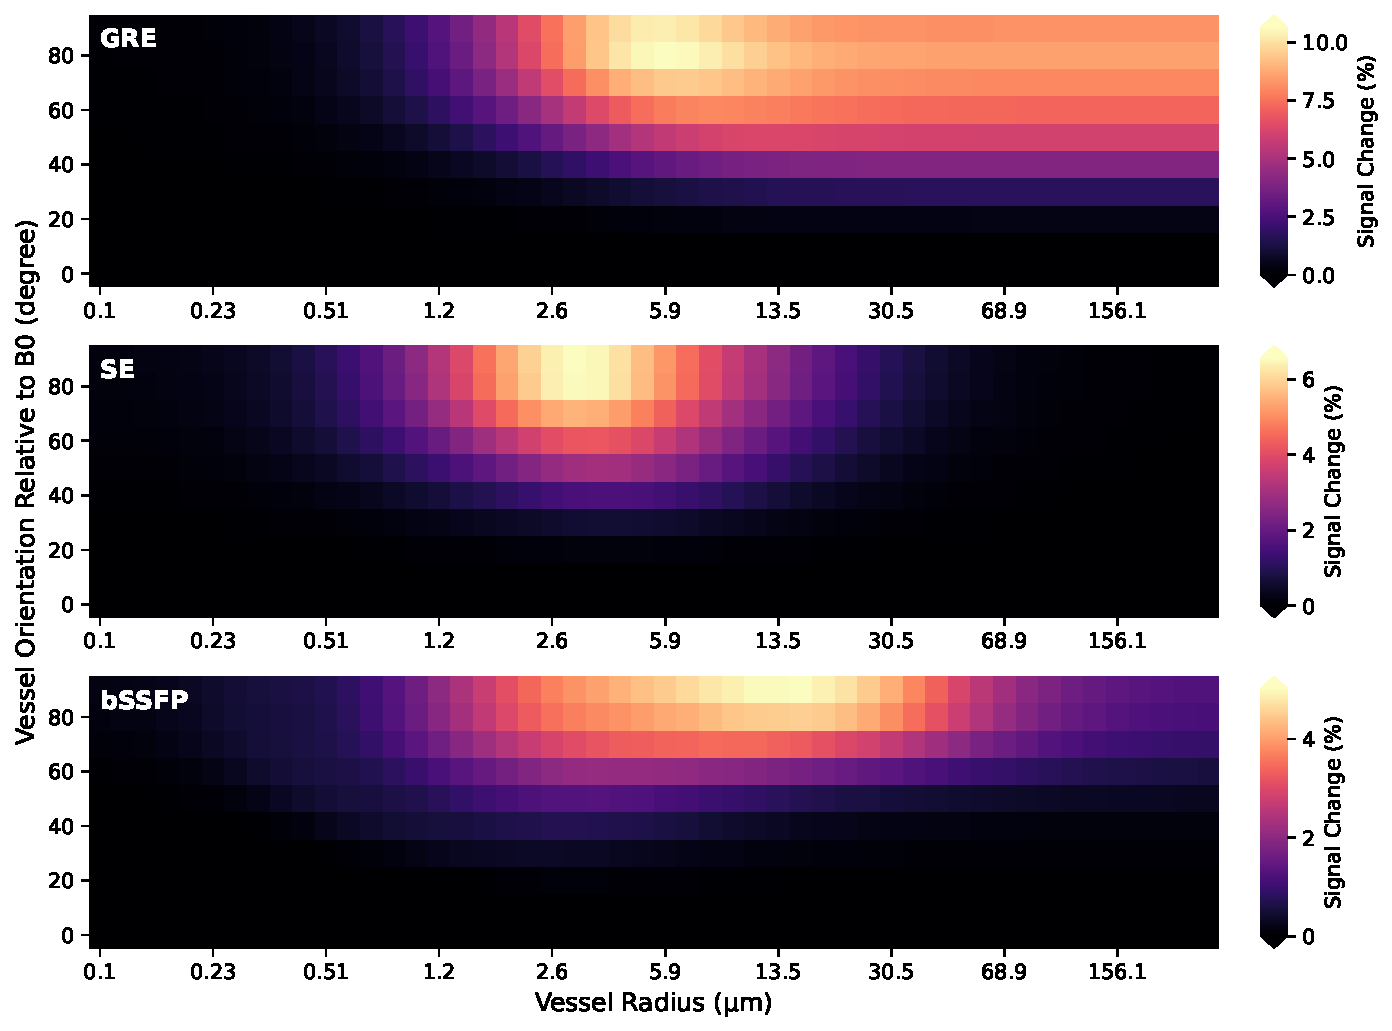
\includegraphics[width=\textwidth]{fig4_orientation.pdf}
    \caption{The extravascular BOLD signal change was analyzed as a function of vessel radius and vessel orientation relative to the B\textsubscript{0} (=9.4\,T) direction under GRE, SE, and bSSFP sequences. Blood oxygenation levels of 77\% for the resting state and 85\% for the activated state were assumed. Phantoms with a FoV of 600 µm, a grid size of 1200, and impermeable surfaces were used, with a blood volume fraction of 4\%. T1 relaxation times were set to 2200\,ms for extravascular and 2500\,ms for intravascular compartments. T2 relaxation times were 41\,ms for extravascular and 13\,ms and 20\,ms for intravascular compartments in the resting and activated states, respectively.}
    \label{fig:orientation}
\end{figure*}
%TC:endignore 

Figure \ref{fig:grase}.A depicts the specificity of a GRASE sequence to vessel sizes. This figure replicates the simulation from Figure 4 in \cite{scheffler2021bold}, with minor adjustments regarding the echo spacing. To maintain consistency with \cite{scheffler2021bold}, the signal change is presented as the difference between active and rest states, rather than as a percentage. This difference is normalized to the number of spins. A total of 19 echoes were acquired, with even echoes being pure SE and odd echoes exhibiting a combination of GRE and SE characteristics. Among the odd echoes, the first echo immediately preceding the refocusing pulse is a pure GRE. As we move to subsequent odd echoes, the SE properties become increasingly evident in the profile (Figure \ref{fig:grase}.B).

%TC:ignore 
\begin{figure*}[!htbp]
    \centering
    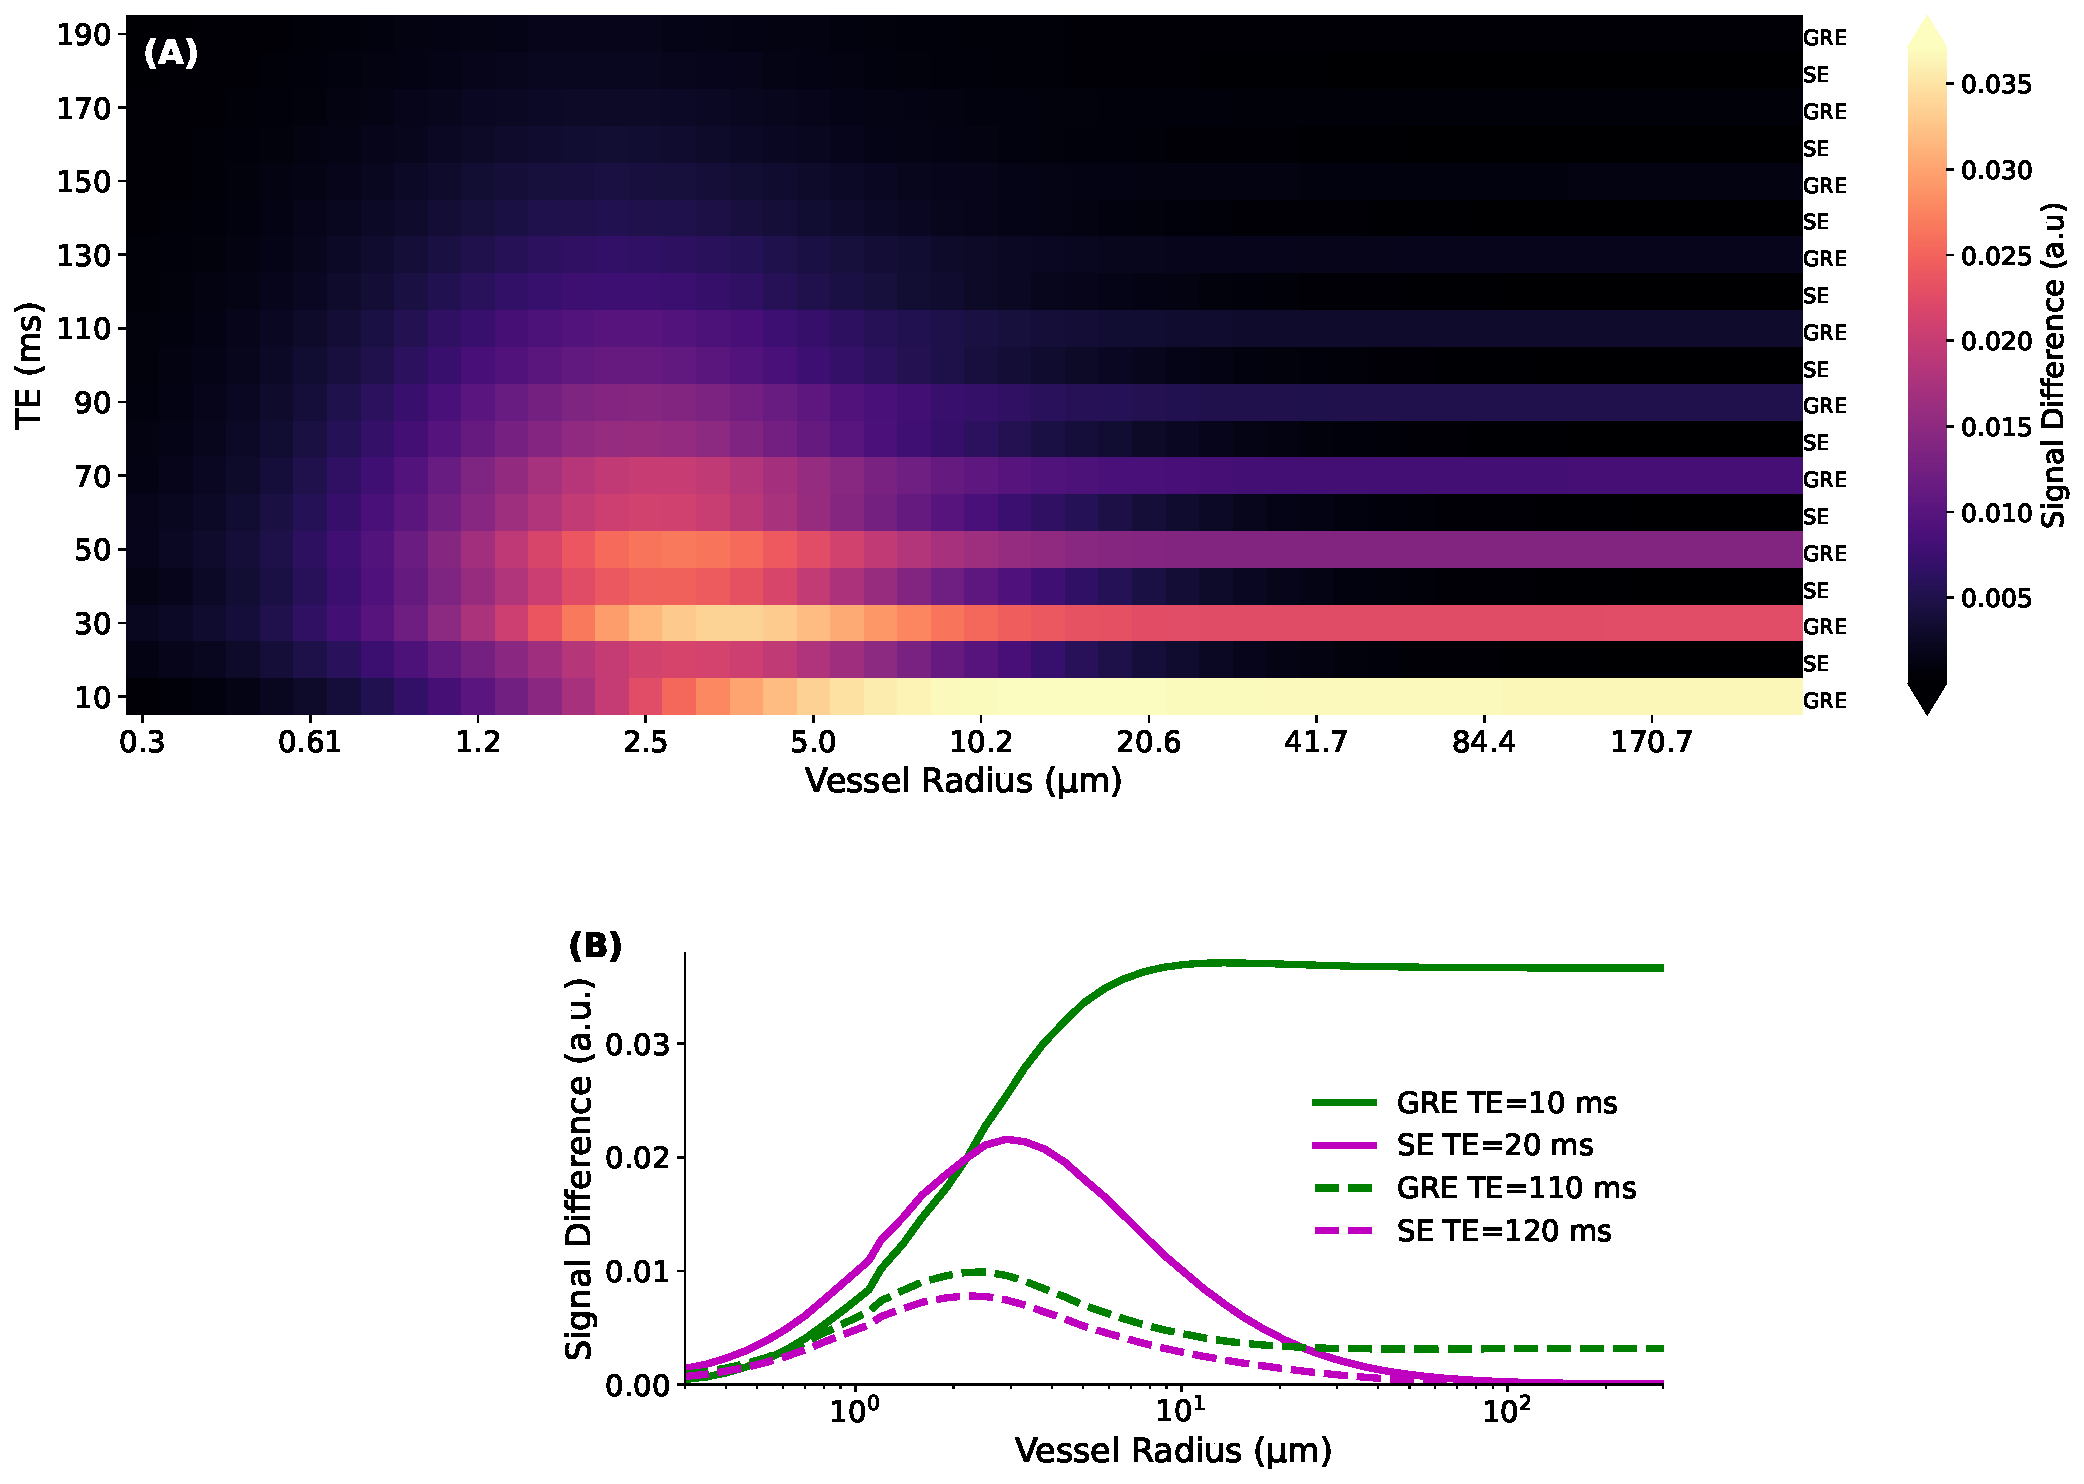
\includegraphics[width=\textwidth]{fig5_grase.pdf}
    \caption{ \textbf{A)} The extravascular BOLD signal change under the GRASE sequence as a function of vessel radius is shown. For consistency with \cite{scheffler2021bold}, the signal change is expressed as the difference between active and rest states and normalized to the number of spins. A total of 19 echoes were collected, with even echoes exhibiting pure SE characteristics and odd echoes displaying a mix of GRE and SE properties. \textbf{B)} The plots show one even (pure SE) and one odd (mix of GRE and SE) echo acquired at both the start and end of the echo train. Notably, the odd echoes, which resemble GRE, gradually exhibit a hybrid profile combining both GRE and SE characteristics as the echo train progresses.}
    \label{fig:grase}
\end{figure*}
%TC:endignore 

Figure \ref{fig:ste} illustrates the effect of mixing time on vessel size specificity in the STE sequence. The primary SE acquired at TE = 40 ms is also shown for reference. The signal change here is also shown as the difference between active and rest states instead of a percentage, to better capture the T\textsubscript{1} relaxation effect. As the mixing time increases, T\textsubscript{1} relaxation becomes more significant, leading to a reduced signal difference between active and rest states. For the examined mixing times, the BOLD signal change is greater than in the SE experiment. When calculated as a percentage, the signal change consistently increases with longer mixing times (results not shown) which is consistent with previously reported simulations and experiments \cite{goerke2006increased}. The simulation indicates that the peak signal shifts towards larger vessels as the mixing time increases.

%TC:ignore 
\begin{figure*}[!htbp]
    \centering
    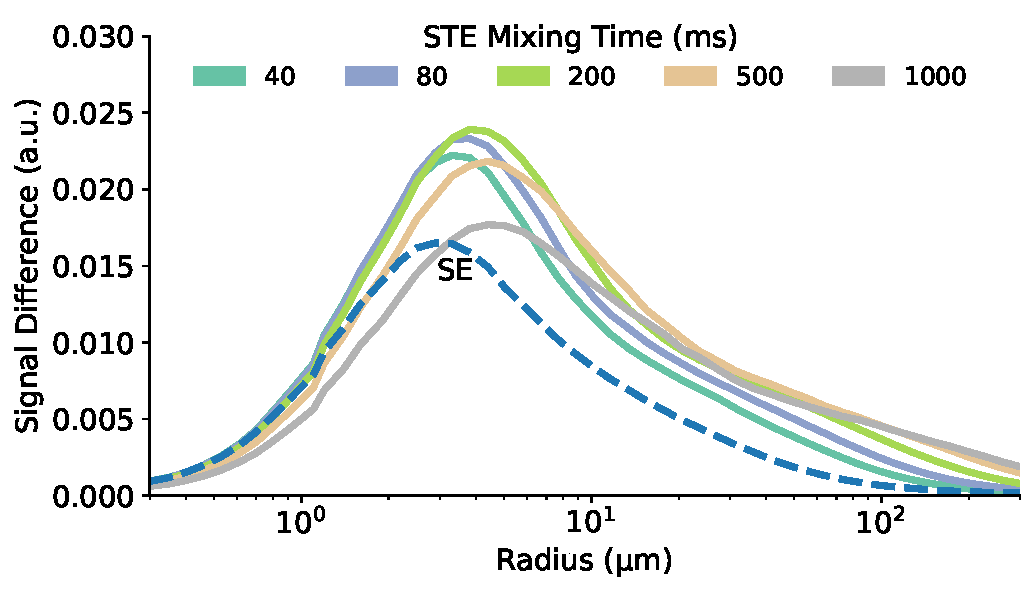
\includegraphics[width=0.75\textwidth]{fig6_ste.pdf}
    \caption{The extravascular BOLD signal changes in the stimulated echo sequence were evaluated as a function of vessel radius and mixing time. The signal change is presented as the difference between active and rest states, rather than as a percentage, to better reflect the T\textsubscript{1} relaxation effect. The results were compared with those from a pure spin echo within the same sequence (dashed line). The initial refocusing RF pulse was applied at 20 ms, generating a spin echo at 40\,ms. The mixing time (T\textsubscript{m}, the interval between the refocusing pulses) was individually examined at 40, 80, 200, 500, and 1000\,ms. }
    \label{fig:ste}
\end{figure*}
%TC:endignore 

Figure \ref{fig:permeability} presents a comparison between impermeable surfaces and 10\% permeability from vessel to tissue in GRE, SE, and bSSFP sequences as a function of vessel radius. Here, 10\% permeability means that when a particle attempts to move from the intravascular to the extravascular space, there is a probability of 10\% that this diffusion will be allowed. It is important to note that in this simulation, the permeability is unidirectional: diffusion from the extravascular to the intravascular space is not permitted. The boundary condition for the FoV that ensures that particles cannot leave the defined simulation area remains enforced throughout the simulations. The simulation indicates that the diffusion of water from the intravascular to the extravascular space can increase the relative signal change in the extravascular space for small vessels in GRE and SE sequences. However, the bSSFP signal behaves differently, with such increases being more pronounced in larger vessels.  Particles in smaller vessels are more likely to diffuse into the extravascular space rapidly, causing their magnetization to reach a steady state well before the signal is acquired at echo-time. In contrast, larger vessels retain some particles that gradually diffuse into the extravascular space closer to echo-time. These particles can retain a memory of their prior presence in the intravascular space, influencing the signal characteristics. Note that in this experiment, the spins that diffuse to the extravascular space are neither replaced nor allowed to diffuse back, which impacts the bSSFP results.

%TC:ignore 
\begin{figure*}[!htbp]
    \centering
    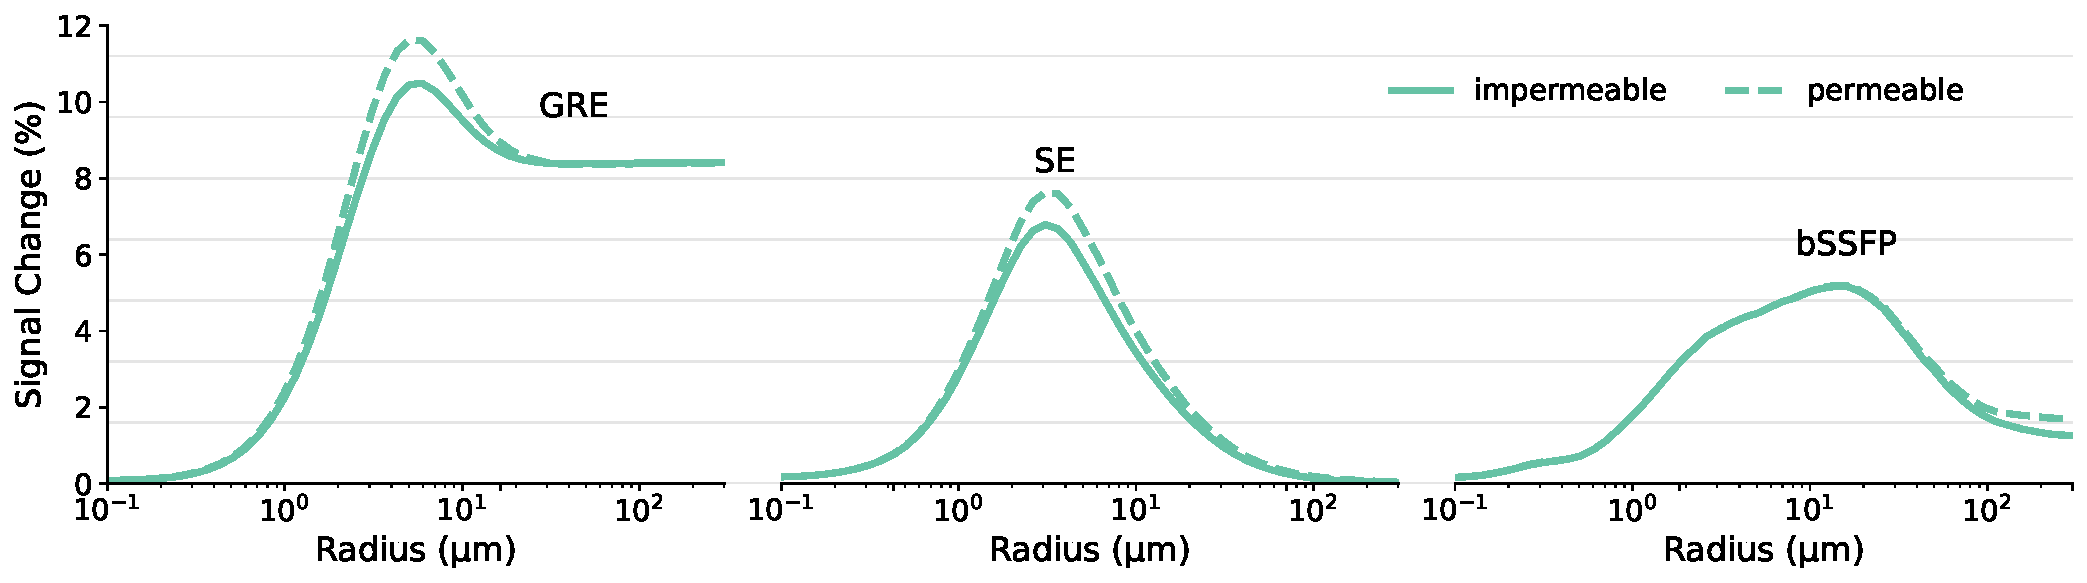
\includegraphics[width=\textwidth]{fig7_permeability.pdf}
    \caption{The effect of permeability, with a probability of 10\% for spins to transfer from intravascular to extravascular compartments, was examined in GRE, SE, and bSSFP sequences as a function of vessel radius. In this context, spins in small vessels are highly likely to contact the vessel surface and exit the substrate if permeability is present. Blood flow is not considered in the simulation, and spins that exit the vessels are neither replaced nor allowed to return. }
    \label{fig:permeability}
\end{figure*}
%TC:endignore 


Figure \ref{fig:diffusion_bias} illustrates how the equilibrium distribution of spins across the substrates can be influenced by changes in diffusivity or the inclusion of permeability in the simulation. When the two substrates have similar diffusivity and permeability conditions, the spin density shows no significant change throughout the entire simulation. However, when the diffusivity of substrate 1 is doubled, spins gradually accumulate in the low diffusivity regions because the mean residence time is longer. As a result, these low diffusivity regions contribute more to the synthesized signals than their volume fraction would suggest. Finally, the introduction of unidirectional permeability—albeit with a small probability—results in a faster reduction of spins in substrate 1. In just one second, more than 10\% of the spins in substrate 1 leave and move into substrate 2.

%TC:ignore 
\begin{figure*}[!htbp]
    \centering
    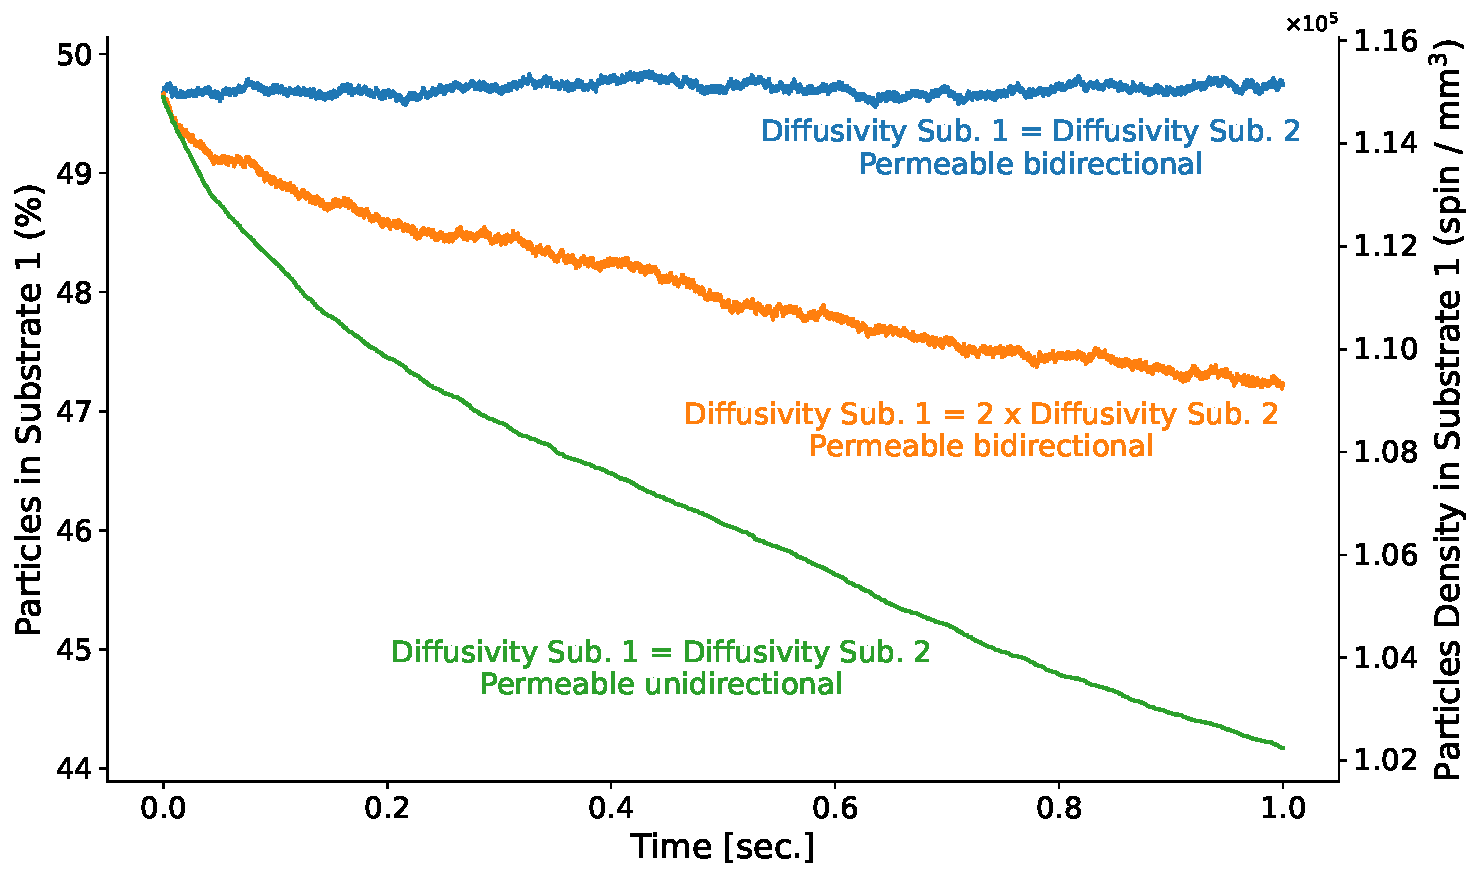
\includegraphics[width=\textwidth]{fig8_diffusion_bias.pdf}
    \caption{The percentage and density of particles remaining in substrate 1 after 1 second of diffusion were analyzed across three scenarios: 1) both substrates had equal diffusivity and the membrane was bidirectionally permeable, 2) substrate 1 had a higher diffusivity than substrate 2, with the membrane still bidirectionally permeable, and 3) both substrates had identical diffusivity, but the permeability was unidirectional, allowing particles to diffuse from substrate 1 to substrate 2 with 10\% probability.}
    \label{fig:diffusion_bias}
\end{figure*}
%TC:endignore 

\subsection*{Computing Performance}

Figure \ref{fig:benchmark} illustrates the performance of SpinWalk when running simulations entirely on a CPU or GPU for 10\textsuperscript{5}, 4x10\textsuperscript{5}, and 10\textsuperscript{6} spins. The study reveals that not only do the number of spins and time steps affect the total simulation time, but the FoV and grid size also play a significant role. These parameters dictate the frequency of memory accesses, a critical factor in GPU computations but of less impact in CPU calculations. The bar plot in Figure \ref{fig:benchmark} demonstrates that, under the conditions tested and with the hardware used, the same simulation can be executed 23 to 78 times faster on a GPU compared to a CPU. Note that the simulations include off-resonance and relaxation effects; without these, the simulations can be expected to run much faster. Also, the values presented in Figure \ref{fig:benchmark} represent the elapsed time for the simulation itself, excluding the initial overhead of loading the phantom and data transfer to DRAM.

The benchmark comparison in the free diffusion experiment among SpinWalk, simDRIFT, and Disimpy shows elapsed times of 1.1, 22, and 35 seconds, respectively, for the simulation of two b-values. For the simulation of 100 b-values, the recorded elapsed times were 53, 46, and 235 seconds for SpinWalk, simDRIFT, and disimpy, respectively. The elapsed times for Disimpy and simDRIFT did not scale 50-fold with a 50-fold increase in the number of b-values. This discrepancy is due to the fact that disimpy and simDRIFT are particularly optimized for diffusion simulations. For instance, simDRIFT reuses a single random walk across all b-values, thereby reducing the number of random number generations required. In contrast, SpinWalk generates a new random walk for each b-value.


%TC:ignore 
\begin{figure*}[!htbp]
    \centering
    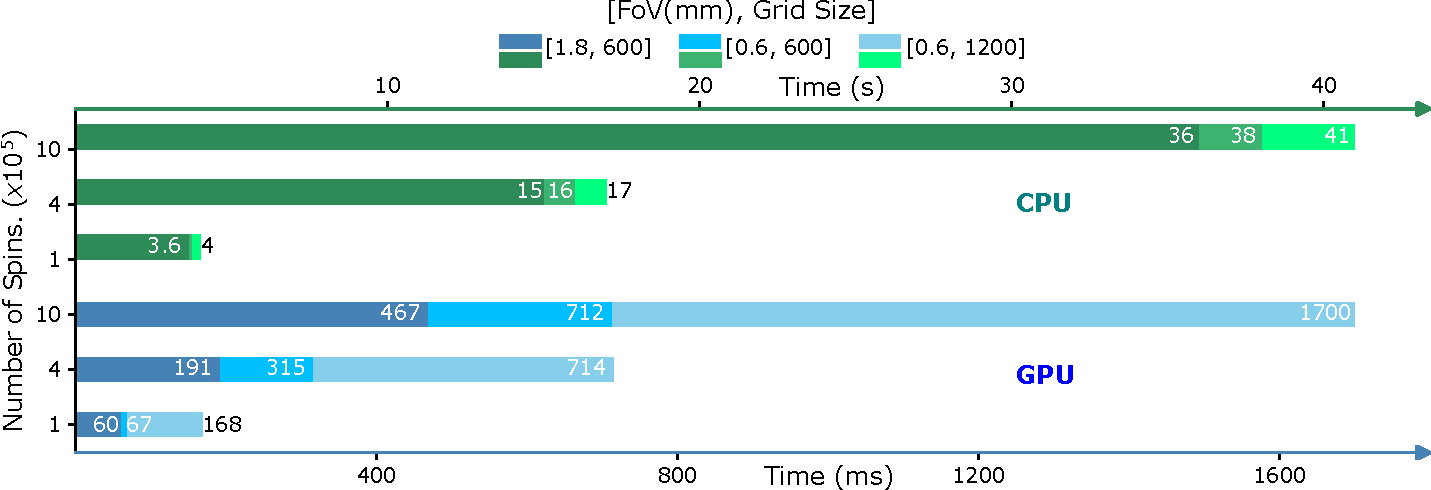
\includegraphics[width=\textwidth]{fig9_benchmark.pdf}
    \caption{The computing performance of SpinWalk was evaluated on both CPU and GPU with respect to the number of spins, phantom FoV, and phantom grid size. The simulation involved 10\textsuperscript{4} random walks of spins in an impermeable environment. The reported elapsed time pertains solely to the simulation itself, excluding the initial overhead associated with loading the phantom and transferring data to DRAM. Notice that the elapsed time is stated in milliseconds for the GPU but in seconds for the CPU for improved visibility.}
    \label{fig:benchmark}
\end{figure*}
%TC:endignore 
